\documentclass[a4paper]{article}

%% Language and font encodings
\usepackage[portuges]{babel}
%\usepackage{fontspec}

%% Sets page size and margins
\usepackage[a4paper,top=3cm,bottom=2cm,left=3cm,right=3cm,marginparwidth=1.75cm]{geometry}

%% Useful packages
\usepackage{amsmath,amsthm,amssymb,amsfonts}
\usepackage{graphicx}
\usepackage[colorinlistoftodos]{todonotes}
\usepackage[colorlinks=true, allcolors=blue]{hyperref}
\usepackage{subfig}
\usepackage{float}



\newcommand{\R}{\mathbb{R}}
\newcommand{\N}{\mathbb{N}}
\newcommand{\Z}{\mathbb{Z}}
\providecommand{\C}{\mathbb{C}}

\theoremstyle{definition}
\newtheorem{defin}{Definição}

\theoremstyle{plain}
\newtheorem{theorem}[defin]{Teorema}
\newtheorem{corollary}[defin]{Corolário}



\title{Laboratório de CEME - Lab 3\\Simulação de de máquina elétrica rotativa}

\author{Cleiton M. Freitas\\
}

\date{}

\begin{document}
\maketitle

%\begin{abstract}
%Your abstract.
%\end{abstract}

%%%%%%%%%%%%%%%%%%%%%%%%%%%%%%%%%%%%%%%%%%
%%%%%%%%%%%%%%%%%%%%%%%%%%%%%%%%%%%%%%%%%%
%%%%%%%%%%%%%%%%%%%%%%%%%%%%%%%%%%%%%%%%%%
\section{Objetivo}

O objetivo desta experiência é analisar o funcionamento de uma máquinas elétrica rotativa a partir de suas equações de fluxo concatenado. Diferentemente dos laboratórios anteriores, a analise conduzida será voltada para a condição de regime permanente.


%%%%%%%%%%%%%%%%%%%%%%%%%%%%%%%%%%%%%%%%%%
%%%%%%%%%%%%%%%%%%%%%%%%%%%%%%%%%%%%%%%%%%
%%%%%%%%%%%%%%%%%%%%%%%%%%%%%%%%%%%%%%%%%%
\section{Máquina Rotativa Analisada}


A máquina elétrica analisada neste semana é conhecida como máquina síncrona. O termo síncrona indica que, para o devido funcionamento dela, deve haver sincronia entre a frequência mecânica de rotação do rotor e a frequência elétrica das tensões e correntes no estator. Além disso, a máquina síncrona possui uma bobina no rotor e esta é alimentada com corrente contínua para produzir o campo magnético principal da máquina~\footnote{Máquinas reais também podem conter outros enrolamentos, chamados de enrolamentos amortecedores, não considerados aqui}. A Figura~\ref{fig:maq} apresenta a vista frontal de uma máquina síncrona com três bobinas do estator, uma para cada fase, e uma bobina no rotor.     


\begin{figure}[H]
\centering
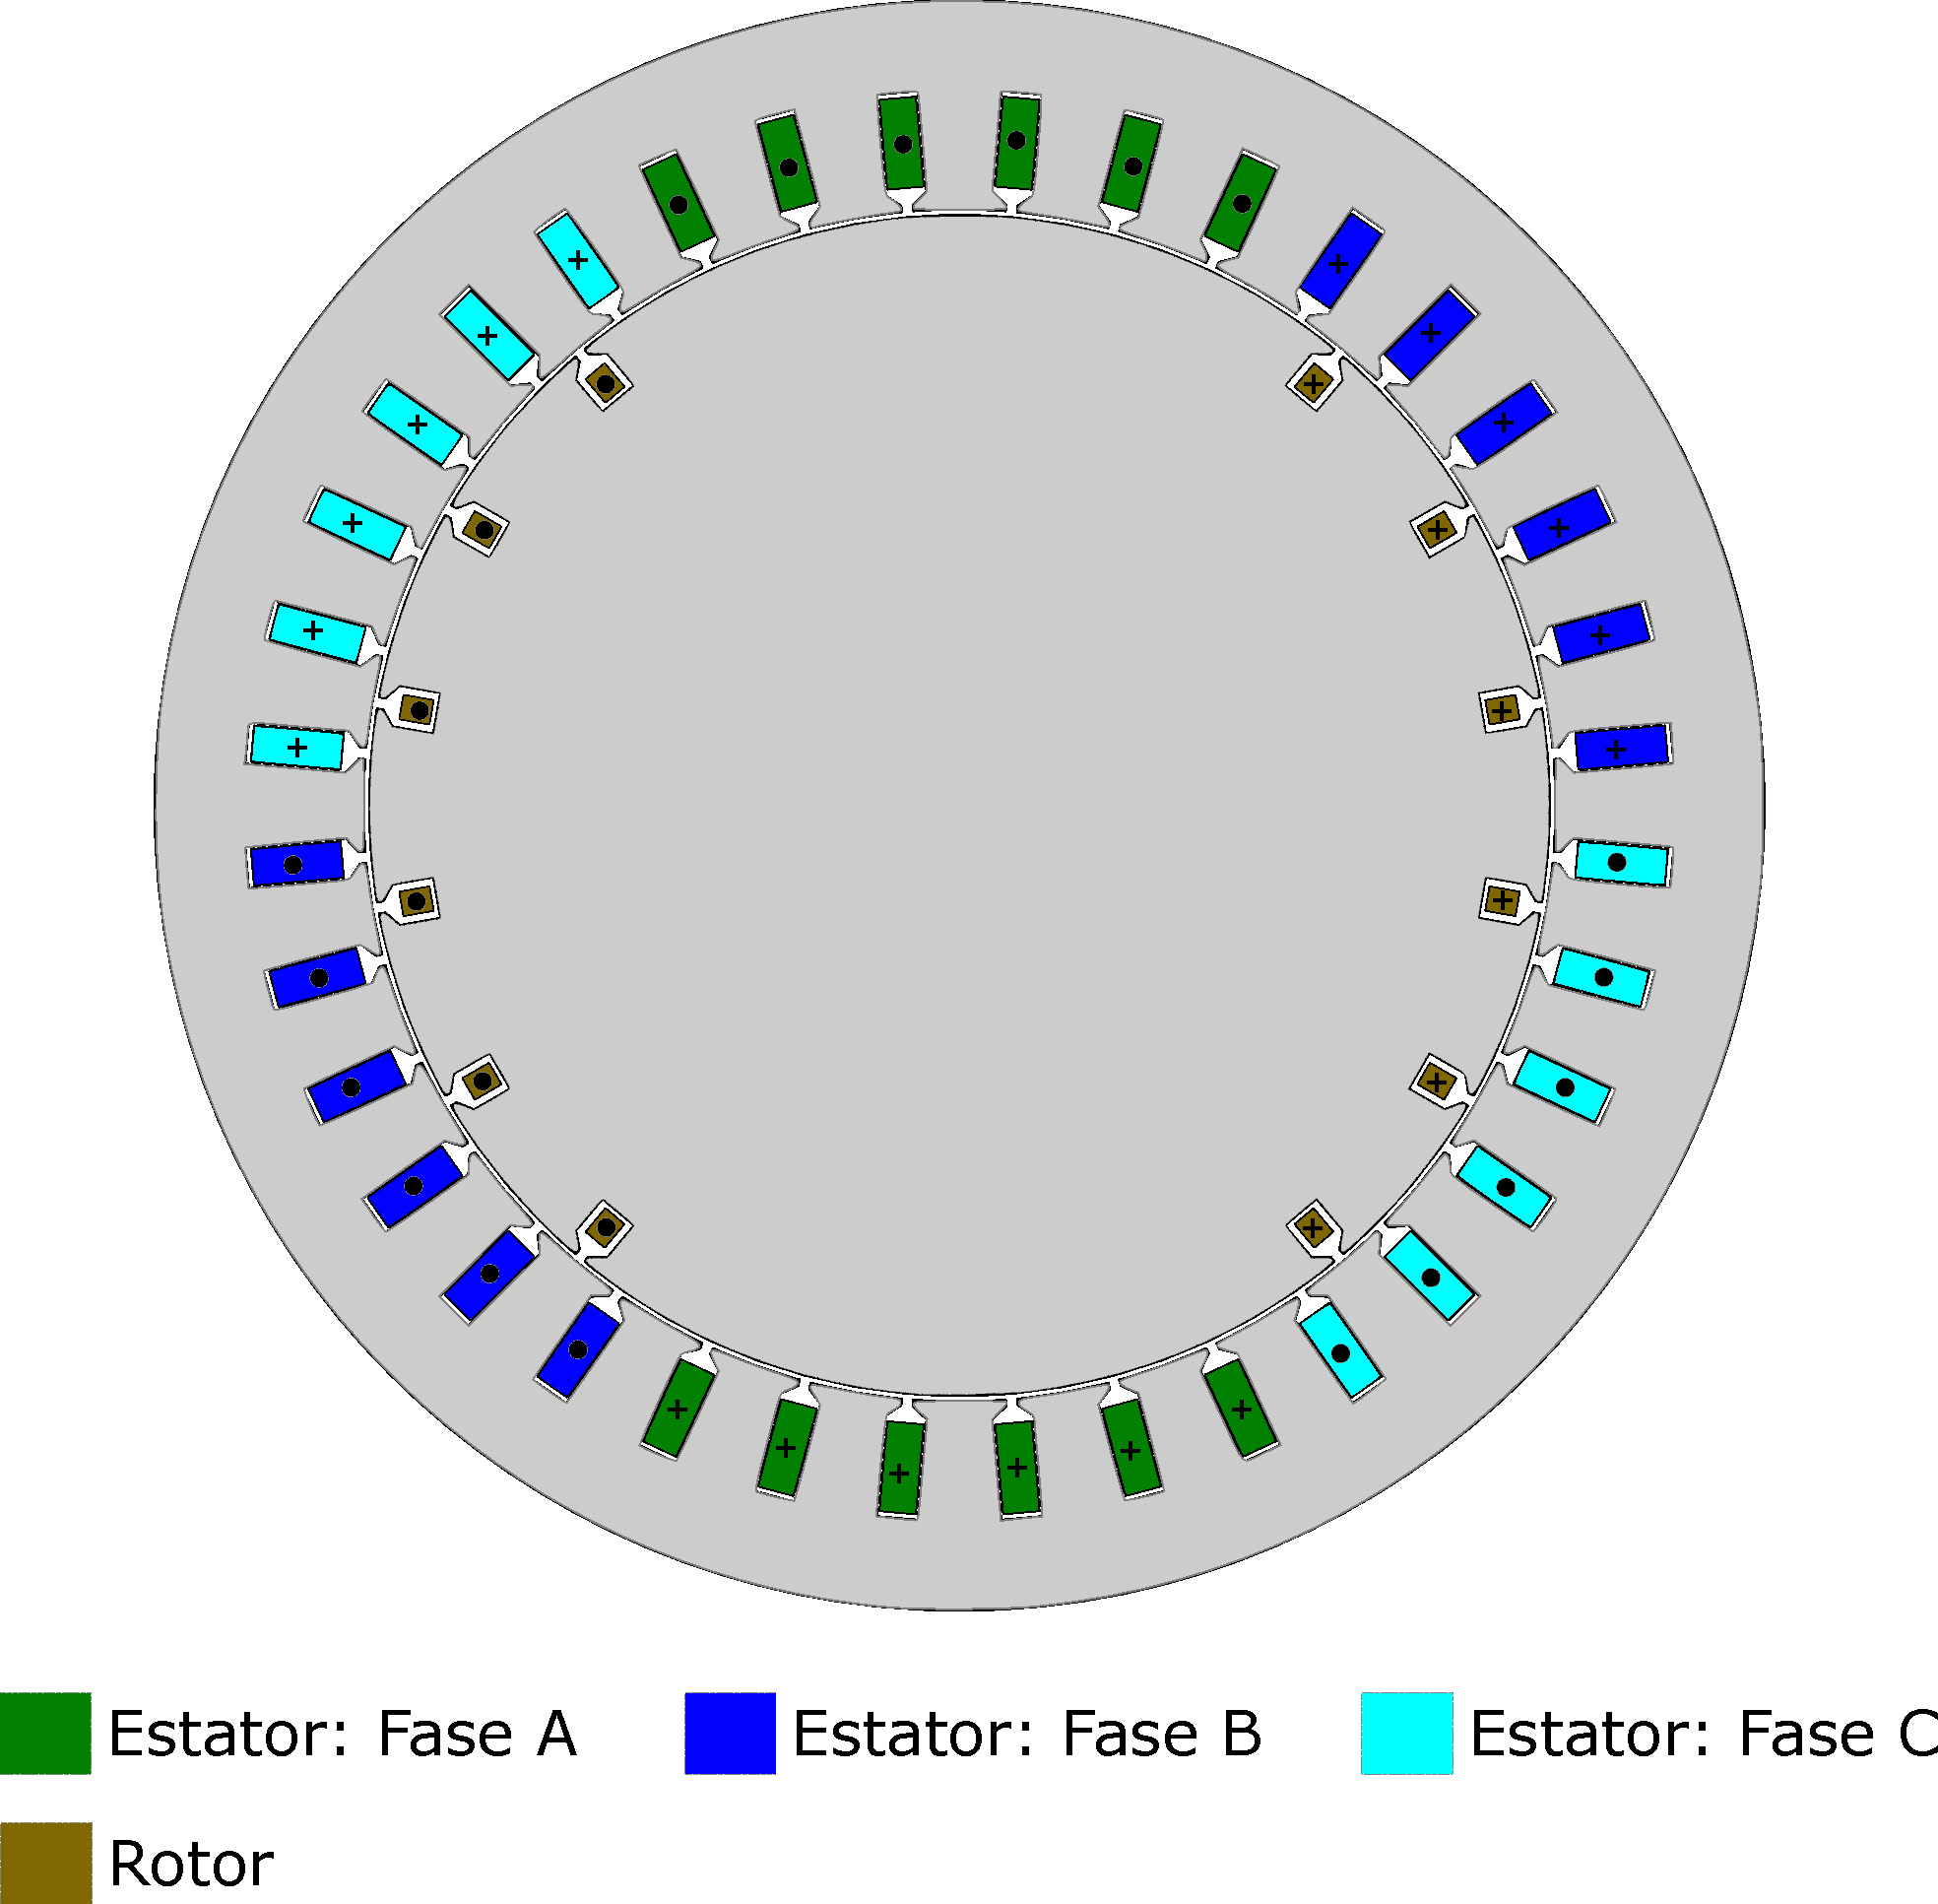
\includegraphics[width=0.75\linewidth]{./figuras/maq_2polos.pdf}
\caption{Máquina síncrona de dois polos}
\label{fig:maq}
\end{figure}



A máquina da Figura~\ref{fig:maq} poder ser descrita pelo seguinte conjunto de equações de fluxo concatenado:


\begin{equation}
\begin{bmatrix}
\lambda_a(t)\\[5pt]
\lambda_b(t)\\[5pt]
\lambda_c(t)\\[5pt]
\lambda_f(t)
\end{bmatrix} =
\begin{bmatrix}
L_{aa} & L_{ab} & L_{ac} & L_{af}\\[5pt]
L_{ba} & L_{bb} & L_{bc} & L_{bf}\\[5pt]
L_{ca} & L_{cb} & L_{cc} & L_{cf}\\[5pt]
L_{da} & L_{fb} & L_{fc} & L_{ff}\\[5pt]
\end{bmatrix}
\begin{bmatrix}
i_a(t)\\[5pt]
i_b(t)\\[5pt]
i_c(t)\\[5pt]
i_f(t)
\end{bmatrix}
\end{equation}
%
onde os subescritos $a$, $b$ e $c$ indicam grandezas referentes as bobinas do estator, enquanto que $f$ indica gradezas relativas a bobina do rotor~\footnote{A bobina do rotor é chamada de bobina de campo, por isso o $f$ de {\it field} geralmente utilizado em livros de máquinas elétricas}.




%%%%%%%%%%%%%%%%%%%%%%%%%%%%%%%%%%%%%%%%%%%
%%%%%%%%%%%%%%%%%%%%%%%%%%%%%%%%%%%%%%%%%%
%%%%%%%%%%%%%%%%%%%%%%%%%%%%%%%%%%%%%%%%%%
\section{Dados do Problema}

A Tabela~\ref{Tab:par} contem os dados construtivos da máquina indicada na Figura~\ref{fig:maq}. Este parâmetros, no entanto, são irrelevantes para as analises que realizaremos.  


\begin{table}[!htb]
\centering
\caption{Parâmetros da máquina rotativa analisada}
\label{Tab:par}
\begin{tabular}{ccc}
\hline
\textbf{Parâmetro}                      & \textbf{Símbolo} & \textbf{Valor} \\ \hline \hline
Distância do Entreferro                 & $g$              & $1mm$          \\
Raio do Rotor                           & $r$              & $9.9cm$        \\
Profundidade                            & $P$              & $15cm$         \\
Número de Espiras por Fase do Estator   & $N_s$            & $72$           \\
Número de Espiras do Rotor              & $N_r$            & $180$          \\
Corrente Nominal das Bobinas do Estator & $I_s$            & $8A_p$         \\
Corrente Nominal das Bobinas do Rotor   & $I_r$            & $2A_p$         \\
Velocidade Nominal da Máquina           & $N$              & $3600RPM$      \\ \hline
\end{tabular}
\end{table}

Com ajuda de um programa voltado para simulação eletromagnética da máquina, o  \href{https://www.femm.info/wiki/HomePage}{FEMM}, foram obtidas as seguintes indutâncias para a máquina: 

\begin{equation}
L_{aa} = L_{bb} = L_{cc} = 0.063 H  
\end{equation}


\begin{equation}
L_{ff} =  0.449 H 
\end{equation}


\begin{equation}
L_{ab} = L_{ac} = L_{bc} = -0.027 H
\end{equation}

\begin{equation}
L_{af} = 0.129 \sin(\theta + 1.57) H
\end{equation}

\begin{equation}
L_{bf} = 0.129 \sin(\theta -0.524) H
\end{equation}

\begin{equation}
L_{cf} = 0.129 \sin(\theta -2.618) H
\end{equation}
%
onde $\theta$ é a posição do rotor da máquina medida me radianos.

%%%%%%%%%%%%%%%%%%%%%%%%%%%%%%%%%%%%%%%%%%%
%%%%%%%%%%%%%%%%%%%%%%%%%%%%%%%%%%%%%%%%%%
%%%%%%%%%%%%%%%%%%%%%%%%%%%%%%%%%%%%%%%%%%
\section{Atividades preliminares}

Considerando as equações de fluxo concatenado, obtenha:

\begin{itemize}
\item As equações para as tensões induzidas de todas as bobinas da máquina
\item O torque eletromagnético em função das correntes e da posição do rotor
\end{itemize}


%%%%%%%%%%%%%%%%%%%%%%%%%%%%%%%%%%%%%%%%%%%
%%%%%%%%%%%%%%%%%%%%%%%%%%%%%%%%%%%%%%%%%%
%%%%%%%%%%%%%%%%%%%%%%%%%%%%%%%%%%%%%%%%%%
\section{Casos Teste}

As próximas subseções apresentam os casos testes que devem ser simulados. Todas as simulações devem ser realizadas no google colab.



%%%%%%%%%%%%%%%%%%%%%%%%%%%%%%%%%%%%%%%%%%
\subsection{Cálculo de tensão induzida: máquina em vazio}

Considerando que:

\begin{itemize}
\item As bobinas do estator estão em vazio (em circuito aberto);
\item A bobina do rotor é alimentada com 2A CC;
\item A máquina é mantida girando a 3600RPM;
\end{itemize}



\begin{enumerate}
\item Plote as tensões induzidas das bobinas
\item A partir dos resultados, determine a frequência e a amplitude das tensões induzidas.
\end{enumerate}




\end{document}